%==============================================================================
% Sjabloon onderzoeksvoorstel bachproef
%==============================================================================
% Gebaseerd op document class `hogent-article'
% zie <https://github.com/HoGentTIN/latex-hogent-article>

% Voor een voorstel in het Engels: voeg de documentclass-optie [english] toe.
% Let op: kan enkel na toestemming van de bachelorproefcoördinator!
\documentclass{hogent-article}

% Invoegen bibliografiebestand
\addbibresource{voorstel.bib}

% Informatie over de opleiding, het vak en soort opdracht
\studyprogramme{Professionele bachelor toegepaste informatica}
\course{Bachelorproef}
\assignmenttype{Onderzoeksvoorstel}


\academicyear{2022-2023}

\title{Scholieren met dyslexie in de derde graad middelbaar onderwijs ondersteunen bij het lezen van wetenschappelijke artikelen via tekstvereenvoudiging.}

\author{Dylan Cluyse}
\email{dylan.cluyse@student.hogent.be}

\supervisor[Co-promotors]{
	\begin{itemize}
		\item J. Decorte (Hogeschool Gent, \href{mailto:johan.decorte@hogent.be}{johan.decorte@hogent.be})
		\item J. Van Damme (Hogeschool Gent, \href{mailto:jana.vandamme@hogent.be}{jana.vandamme@hogent.be})
	\end{itemize} 
% M. Dhondt (Gelukstraat \href{mailto:marloesdhondt@gelukstraat.be}{marloesdhondt@gelukstraat.be})
}

\specialisation{AI \& Data Engineering}
\keywords{Machineleertechnieken en kunstmatige intelligentie, tekstvereenvoudiging, dyslexie}
\begin{document}
	
\begin{abstract}
% nood van de doelgroep
% --> iets uit de literatuur gebruiken om te starten --> afbakenen
% noden aftoetsen aan wat er bestaat --> geautomatiseerd om breder toegankelijk te maken binnen het onderwijs
% Hoe kan de inhoud ... --> Hoe kan een wetenschappelijk artikel
% bovenschikking --> onderschikking
Ingewikkelde woordenschat en zinsbouw hinderen scholieren met dyslexie in het derde graad middelbaar onderwijs bij het lezen van wetenschappelijke artikelen. Gepersonaliseerde automated text simplification (ATS) helpt deze scholieren bij hun leesbegrip. Daarnaast kan artificiële intelligentie (AI) dit proces automatise- ren om de werkdruk bij leraren en scholieren te verminderen. Dit onderzoek ach- terhaalt met welke technologische en logopedische aspecten AI-ontwikkelaars re- kening moeten houden bij de ontwikkeling van een AI-toepassing voor geauto- matiseerde en gepersonaliseerde tekstvereenvoudiging. Hiervoor is de volgende onderzoeksvraag opgesteld: ”Hoe kan een wetenschappelijk artikel automatisch worden vereenvoudigd, gericht op de unieke noden van scholieren met dyslexie in de derde graad middelbaar onderwijs?”. Een requirementsanalyse achterhaalt de benodigde functionaliteiten om gepersonaliseerde en geautomatiseerde tekst- vereenvoudiging mogelijk te maken. Vervolgens wijst de vergelijkende studie uit welk taalmodel het meest inzetbaar is om de taak van gepersonaliseerde en geau- tomatiseerde tekstvereenvoudiging mogelijk te maken. De requirementsanalyse wijst uit dat toepassingen om wetenschappelijke artikelen te vereenvoudigen, zich richten op een centrale doelgroep en geen rekening houden met de unieke noden van een scholier met dyslexie in de derde graad middelbaar onderwijs. Toe- passingen voor gepersonaliseerde ATS zijn mogelijk, maar ontwikkelaars moeten meer inzetten op de unieke noden van deze scholieren. 
\end{abstract}

% oplijsting kunnen beantwoorden: wat zit er nu nog niet in een applicatie?

\tableofcontents

%---------- Inleiding ---------------------------------------------------------

\section{Introductie}%
\label{sec:introductie}

% Met een jaarlijks budget van 32 miljoen in het vakgebied kunstmatige intelligentie (AI) op de werkvloer is België een pionier \autocite{Crevits2022}.  Zo zijn er verschillende projecten, om taalgerelateerde AI-ontwikkelingen op te starten, uit de grond gestampt. Het amai!-project \footnote{https://amai.vlaanderen/}  verenigt AI-softwarebedrijven uit verschillende domeinen om zo met AI-toepassingen te maken die processen automatiseren om de werkdruk te verminderen, zoals binnen het onderwijs \textit{real-time} ondertiteling en een taalassistent voor leerkrachten in meertalige klasgroepen.

Het Vlaams middelbaar onderwijs staat op barsten. Werkdruk en stress overspoelen leraren en scholieren. Bovendien is de derde graad van het middelbaar onderwijs een belangrijke mijlpaal voor de verdere loopbaan van scholieren, al hebben zij volgens \textcite{Dapaah2022} dan moeite om grip te krijgen op de vakliteratuur bij STEM-vakken. De STEM-agenda\footnote{https://www.vlaanderen.be/publicaties/stem-agenda-2030-stem-competenties-voor-een-toekomst-en-missiegericht-beleid} van de Vlaamse overheid moet het STEM-onderwijs tegen 2030 aantrekkelijker te maken, door de ondersteuning voor zowel leerkrachten als scholieren te verbeteren. Toch neemt deze agenda de aanpak van steeds complexere wetenschappelijke taal, zoals beschreven in \textcite{Barnett2020}, niet op. Wetenschappelijke artikelen vereenvoudigen, op maat van de noden van een scholier met dyslexie in het middelbaar onderwijs, is tijds- en energie-intensief voor leerkrachten en scholieren. Automatische en adaptieve tekstvereenvoudiging biedt hier een baanbrekende oplossing om de werkdruk in het middelbaar onderwijs te verminderen.

Het doel van dit onderzoek is om te achterhalen met welke technologische en logopedische aspecten AI-ontwikkelaars rekening moeten houden bij de ontwikkeling van een adaptieve AI-toepassing voor geautomatiseerde tekstvereenvoudiging. De volgende onderzoeksvraag is opgesteld: "Hoe kan een wetenschappelijk artikel automatisch vereenvoudigd worden, gericht op de verschillende behoeften van scholieren met dyslexie in de derde graad middelbaar onderwijs?". Een antwoord op volgende deelvragen kan de onderzoeksvraag vereenvoudigen. Eerst geeft de literatuurstudie een antwoord op de eerste vier deelvragen. Daarna vormt het veldonderzoek een antwoord op de vijfde deelvraag. Ten slotte beantwoordt de vergelijkende studie de zesde en laatste deelvraag. De resultaten van dit onderzoek zetten AI-ontwikkelaars aan om een toepassing te maken om scholieren met dyslexie te kunnen ondersteunen in de derde graad middelbaar onderwijs.

% wat wordt manueel gedaan? --> voor de doelgroep
 % --> kleiner prototype
  
% aantal deelvragen doet er niet toe, maak gewoon dat je concrete en doelgerichte deelvragen hebt

\begin{enumerate}
	\item Welke aanpakken zijn er voor geautomatiseerde tekstvereenvoudiging? Aansluitende vraag: "Hoe worden teksten handmatig vereenvoudigd voor scholieren met dyslexie?"
	\item Welke specifieke noden hebben scholieren van de derde graad middelbaar onderwijs bij het begrijpen van complexere teksten?
	\item Wat zijn de specifieke kenmerken van wetenschappelijke artikelen? 
	\item Met welke valkuilen bij taalverwerking met AI moeten ontwikkelaars rekening houden?
	\item Welke toepassingen, tools en modellen zijn er beschikbaar om Nederlandstalige geautomatiseerde tekstvereenvoudiging met AI mogelijk te maken?
	\item Welke functies ontbreken AI-toepassingen om geautomatiseerde én adaptieve tekstvereenvoudiging mogelijk te maken voor \newline scholieren met dyslexie in de derde graad \newline middelbaar onderwijs? Aansluitende vraag: "Welke manuele methoden voor tekstvereenvoudiging komen niet in deze tools voor?"
\end{enumerate}

%---------- Stand van zaken ---------------------------------------------------

\section{State-of-the-art}%
\label{sec:state-of-the-art}

\subsection{Tekstvereenvoudiging}

% Deelvraag: Wat is tekstsimplificatie
De voorbije tien jaar is artificiële intelligentie (AI) sterk verder ontwikkeld. \textcite{Vasista2022} benadrukt dat de toename in kennis voor nieuwe toepassingen zorgde. Tekstvereenvoudiging vloeide hier uit voort. Momenteel bestaan er al robuuste toepassingen die teksten kunnen vereenvoudigen, zoals Resoomer\footnote{https://resoomer.com/nl/}, Paraphraser\footnote{https://www.paraphraser.io/nl/tekst-samenvatting} en Prepostseo\footnote{https://www.prepostseo.com/tool/nl/text-summarizer}. Binnen het kader van tekstvereenvoudiging is er bestaande documentatie beschikbaar waar onderzoekers het voordeel van toegankelijkheid aanhalen, maar volgens \textcite{Gooding2022} ontbreken deze toepassingen de extra noden die scholieren met dyslexie in de derde graad middelbaar onderwijs vereisen.

\textcite{Shardlow2014} haalt aan dat het algemene doel van tekstvereenvoudiging is om ingewikkelde bronnen toegankelijker te maken. Het zorgt voor verkorte teksten zonder de kernboodschap te verliezen. \textcite{Siddharthan2014} haalt verder aan dat tekstvereenvoudiging op één van drie manieren gebeurt. Er is conceptuele vereenvoudiging waarbij documenten naar een compacter formaat worden getransformeerd. Daarnaast is er uitgebreide modificatie die kernwoorden aanduidt door gebruik van redundantie. Als laatste is er samenvatting die documenten verandert in kortere teksten met alleen de topische zinnen. Met deze concepten zijn ontwikkelaars volgens \textcite{Siddharthan2014} in staat om ingewikkelde woorden te vervangen door eenvoudigere synoniemen of zinnen te verkorten zodat ze sneller leesbaar zijn.

Tekstvereenvoudiging behoort tot de zijtak van \textit{Natural Language Processing} (NLP) in AI. NLP omvat methodes om menselijke teksten om te zetten in tekst voor machines. Documenten vereenvoudigen met NLP kan volgens \textcite{Chowdhary2020} op twee manieren: extraherend of abstraherend. Bij extraherende vereenvoudiging worden zinnen gelezen zoals ze zijn neergeschreven. Vervolgens bewaart een document de belangrijkste taalelementen om de tekst te kunnen hervormen. Deze vorm van tekstvereenvoudiging komt volgens \autocite{Sciforce2020} het meeste voor. Daarnaast is er abstraherende vereenvoudiging waarbij de kernboodschap wordt bewaard. Met de kernboodschap wordt er een nieuwe zin opgebouwd. Volgens het onderzoek van \textcite{Chowdhary2020} heeft deze vorm potentieel, maar het zit nog in de kinderschoenen.

\subsection{Noden van scholieren met dyslexie}

% Deelvraag 2: Bewezen voordelen van tekstsimplificatie bij scholieren met dyslexie
Het experiment van Franse wetenschappers \newline \textcite{Gala2016} illustreert dat manuele tekstvereenvoudiging schoolteksten toegankelijker \newline maakt voor kinderen met dyslexie. Dit deden ze door simpelere synoniemen en zinsstructuren te gebruiken. Tien kinderen werden opgenomen in het experiment, variërend van 8 tot 12 jaar oud. Verwijswoorden werden vermeden en woorden kort gehouden. De resultaten waren veelbelovend. Het leestempo lag hoger en de kinderen maakten minder leesfouten. Ook bleek er geen verlies van begrip in de tekst bij geteste kinderen. Resultaten van de studie werden gebundeld voor de mogelijke ontwikkeling van een AI-tool.

% doelgroep concreter maken hierboven
% semantisch vlak --> zinsstructuur
% welke criteria vonden zij 'geslaagd'?

De visuele weergave van tekst beïnvloedt de leessnelheid bij scholieren met dyslexie. Zo haalt het onderzoek van \textcite{Rello2012} tips aan waarmee teksten en documenten rekening moeten houden bij scholieren met dyslexie in de derde graad middelbaar onderwijs. Het gaat over speciale lettertypes, spreiding tussen woorden en het gebruik van inzoomen op aparte zinnen. Het onderzoek haalt verder aan dat teksten voor deze unieke noden aanpassen tijdrovend is en daarmee tekstvereenvoudiging door AI een revolutionaire oplossing kan bieden. De Universiteit van Kopenhagen is met bovenstaande idee aan de slag gegaan. Onderzoekers \textcite{Bingel2018} hebben gratis software ontwikkeld, genaamd Hero\footnote{https://beta.heroapp.ai/}, om tekstvereenvoudiging voor scholieren in het middelbaar onderwijs met dyslexie te automatiseren. De software bestudeert met welke woorden de gebruiker moeite heeft, en vervangt die door simpelere alternatieven. Hero bevindt zich nu in beta-vorm en wordt enkel in het Engels en Deens ondersteund. Als alternatief is er Readable\footnote{https://readable.com/}. Dit is een Engelstalige AI-toepassing dat zinnen beoordeeld met leesbaarheidsformules.

% Deelvraag: Uitdagingen van AI-software met tekstsimplificatie
\textcite{Roldos2020} haalt aan dat NLP in de laatste decennia volop in ontwikkeling is, maar ontwikkelaars botsen nog op uitdagingen. Het gaat om zowel interpretatie- als dataproblemen bij AI-modellen. Het onderzoek haalt twee punten aan. Allereerst is het voor een machine moeilijk om de context van homoniemen te achterhalen. Bijvoorbeeld bij het woord ‘bank’ is het niet duidelijk voor de machine of het gaat over de geldinstelling of het meubel. Daarnaast zijn synoniemen een probleem voor tekstverwerking.

Het onderzoek van \textcite{Sciforce2020} haalt aan dat het merendeel van NLP-toepassingen Engelstalige invoer gebruikt. Niet-Engelstalige toepassingen zijn zeldzaam. De opkomst van AI technologieën die twee datasets gebruiken, biedt een oplossing voor dit probleem. De software vertaalt eerst de oorspronkelijke tekst naar de gewenste taal, voordat de tekst wordt herwerkt. Hetzelfde onderzoek bewijst dat het vertalen van gelijkaardige talen, zoals Duits en Nederlands, een minimaal verschil opleverd.

% Deelvraag: Stand van zaken bij Belgische secundaire scholen
% Voor scholieren met dyslexie in het derde graad middelbaar onderwijs bestaan digitale hulpmiddelen die voor een betere visuele presentatie zorgen van teksten. De Vlaamse overheid leent gratis abonnementen\footnote{https://onderwijs.vlaanderen.be/nl/onderwijspersoneel/van-basis-tot-volwassenenonderwijs/lespraktijk/ict-in-de-klas/voorleessoftware-voor-leerlingen-met-leesbeperkingen} uit voor voorlees- en schrijfsoftware. De voornaamste zijn SprintPlus\footnote{https://www.sprintplus.be/}, Alinea\footnote{https://sensotec.be/product/alinea-suite/} en Kurzweil3000\footnote{https://sensotec.be/product/kurzweil-3000/}. Vlaamse scholieren met dyslexie in het middelbaar onderwijs kunnen voor deze software een gratis abonnement of licentie aanvragen. Al bieden de vijf softwarepakketten elk een samenvattingsfunctie aan, echter ligt de focus op spreek- en luisterfuncties waarbij het samenvatten en markeren van tekst als extra wordt gehouden.

% \subsection{Wetenschappelijke artikelen}

Volgens \textcite{PlavenSigray2017} houden onderzoekers zich vaak in hun eigen taalbubbel, wat negatieve gevolgen heeft voor de leesbaarheid van een wetenschappelijk artikel. Bovendien vormt de stijgende trend van het gebruik aan acroniemen \textcite{Barnett2020} een extra hindernis. \textcite{Donato2022} haalt aan dat onbegrijpelijke literatuur, waaronder studiemateriaal geschreven door de docent en online wetenschappelijke artikelen, één van de redenen is waarom scholieren met dyslexie in het middelbaar onderwijs van richting veranderen.

\subsection{Huidige toepassingen}

Vlaanderen heeft weinig zicht op de geïmplementeerde AI software in scholen. Dit werd vastgesteld door \autocite{Martens2021}, een samenwerking tussen de Vlaamse universiteiten en overheid voor AI. Vergeleken met andere Europese landen, maakt België het minst gebruik van leerling-georiënteerde hulpmiddelen. Degenen die wel gebruikt worden, zijn vooral online leerplatformen voor zelfstandig werken. Ook maakt België amper gebruik van beschikbare software die de leermethoden en -noden van leerlingen evalueert \autocite{Martens2021a}. 

\textcite{Verhoeven2023} haalt aan dat AI-toepassingen zoals ChatGPT, Google Bard en Bing AI kunnen helpen om routinematig werk te verminderen in het onderwijs. Echter haalt \textcite{Deckmyn2021} aan dat GPT-3, het model van ChatGPT, sterker staat in het maken van Engelstalige teksten vergeleken met Nederlandstalige teksten. De databank waar het GPT-3 model mee is getraind, bestaat uit 92\% Engelstalige woorden, terwijl er 0,35\% Nederlandse woorden aanwezig zijn in dezelfde databank. Ontwikkelaars moeten de evolutie van deze modellen opvolgen, voordat er Nederlandstalige toepassingen mee worden gemaakt.

% eventueel Bing AI bekijken
% --> artikel: 

% Deelvraag: Wat is er nodig voor tekstsimplificatie? 

\subsection{Ontwikkelen met AI}

Python staat bovenaan de lijst van programmeertalen voor NLP-toepassingen. Volgens het onderzoek van \textcite{Thangarajah2019} is dit te wijten aan de eenvoudige syntax, kleine leercurve en grote beschikbaarheid van kant-en-klare bibliotheken. Wiskundige berekeningen of statistische analyses kunnen worden uitgevoerd met één lijn code. \textcite{Malik2022} haalt de twee meest voorkomende aan, namelijk NLTK\footnote{https://www.nltk.org/} en Spacy\footnote{https://spacy.io/}. \textit{Deep Martin}\footnote{https://github.com/chrislemke/deep-martin} bouwt verder op het onderzoek van \textcite{Shardlow2014} naar een pipeline voor lexicale vereenvoudiging. \textit{Deep Martin} maakt gebruik van \textit{custom transformers} om invoertekst te converteren naar een vereenvoudigde versie van de tekstinhoud.

Voor Germaanse talen zijn er enkele datasets en word embeddings beschikbaar die de complexiteit van woorden bijhouden. Zo zijn er in de Duitse taal Klexicon\footnote{https://github.com/dennlinger/klexikon} en TextComplexityDE\footnote{https://github.com/babaknaderi/TextComplexityDE}. Een onderzoek van \textcite{Suter2016} bouwde een rule-based NLP-model met 'Leichte Sprache', wat een dataset is met eenvoudige Duitstalige zinsconstructies. Nederlandstalige datasets zijn in schaarse hoeveelheden beschikbaar, waardoor het vertalen uit een Germaanse taal is hier een optie.

Volgens \textcite{Garbacea2021} is het belangrijk dat AI-ontwikkelaars niet alleen aandacht besteden aan het aanpassen van woorden en zinnen, maar ook aan de gebruiker meegeven waarom iets is aangepast. De onderzoekers wijzen op twee ethische aspecten. Eerst moet de toepassing duidelijk aangeven waarom een woord of zin is aangepast. Het model moet de moeilijkheidsgraad van de woorden of zinnen bewijzen. \textcite{Iavarone2021} beschrijft een methode met regressiemodellen om de moeilijkheidsgraad te bepalen door een gemiddeld moeilijkheidspercentage per zin te berekenen. Daarnaast benadrukt \textcite{Garbacea2021} het belang van het markeren van de complexere delen van een tekst. Hiervoor haalt hetzelfde onderzoek methoden aan zoals \textit{lexical} of \textit{deep learning}.

Er is een tactvolle aanpak nodig om een vereenvoudigde tekst met AI te beoordelen. De studie van \textcite{Swayamdipta2019} haalt aan dat er extra nood is aan NLP-modellen waarbij de tekst zijn kernboodschap behoudt. Samen met Microsoft Research bouwden ze NLP-modellen die gericht waren op de bewaring van zinsstructuur en -context door \emph{scaffolded learning}. Hiervoor maakten de onderzoekers gebruik van een voorspellingsmethode die de positie van woorden en zinnen in een document beoordeelde. De Flesch-Kincaid leesbaarheidstest is volgens \newline \textcite{Readable2021} een alternatieve manier om vereenvoudigde tekstinhoud te beoordelen, zonder de nood aan \textit{pre-trained} modellen. Figuur \ref{img:readable-scheme} geeft de indeling per doelgroep weer. Deze score kan eenvoudig worden berekend met de \textit{Python-library} \textit{textstat}\footnote{https://pypi.org/project/textstat/}. 

\begin{figure}
	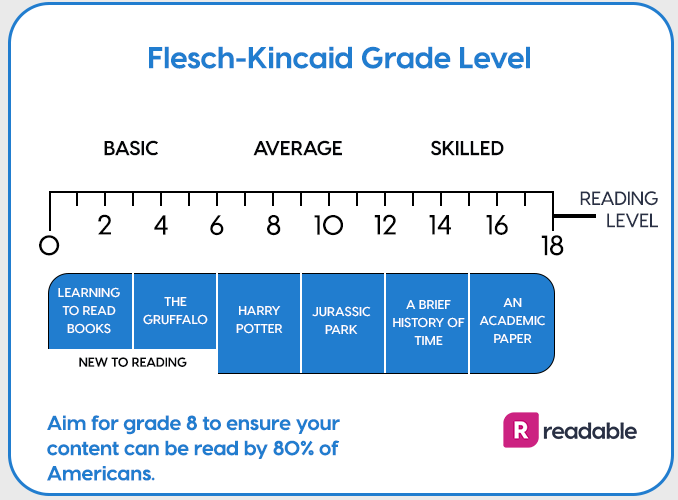
\includegraphics[width=\linewidth]{img/Screenshot_302.png}
	\caption{De indeling van leesgraadscores per doelgroep. Bron: \autocite{Readable2021}}
	\label{img:readable-scheme}
\end{figure}

%---------- Methodologie ------------------------------------------------------
\section{Methodologie}%
\label{sec:methodologie}
Een \textit{mixed-methods} onderzoek toont aan hoe toepassingen automatisch een wetenschappelijke artikel kunnen vereenvoudigen, gericht op scholieren met dyslexie in de derde graad middelbaar onderwijs. Het onderzoek houdt vijf grote fases in. De eerste fase is het proces van geautomatiseerde tekstvereenvoudiging beschrijven. Dit gebeurt via een grondige studie van vakliteratuur en wetenschappelijke teksten. Ook blogs van experten komen hier aan bod. Na het verwerven van de nodige inzichten wordt er een verklarende tekst opgesteld.

De tweede fase bestaat uit het analyseren van wetenschappelijke werken over de bewezen voordelen van tekstvereenvoudiging bij scholieren met dyslexie van de derde graad middelbaar onderwijs. Hiervoor zijn geringe thesissen beschikbaar, die zorgvuldigheid vragen tijdens interpretatie. De resulterende tekst bevat de voordelen samen met hun wetenschappelijke onderbouwing.

De derde fase is opnieuw een beschrijving. Hier worden de valkuilen bij taalverwerking met AI-software nagegaan. Deze fase van het onderzoek brengt mogelijke nadelen en tekortkomingen van AI-software bij tekstvereenvoudiging aan het licht. Dit gebeurt aan de hand van een technische uitleg.

De vierde fase omvat een toelichting over beschikbare AI toepassingen voor tekstvereenvoudiging. Aan de hand van een veldonderzoek op het internet en bij bedrijven wordt een longlist opgesteld van beschikbare toepassingen voor tekstvereenvoudiging in het middelbaar onderwijs. Met een requirementsanalyse wordt er een shortlist opgesteld van software. Het toetsen van verschillende tools wordt ook betrokken in deze fase. De shortlist vormt de basis voor de ontwikkeling van een prototype voor geautomatiseerde en adaptieve tekstvereenvoudiging.

% bestaande technologie gebruiken
% multilinguale modellen --> Nederlands als brugtaal
% hoe testen? --> output van specifieke tools
% trials --> selectie van maken --> als ik 'dit' toepas, dan krijg ik 'dit'

% tool van nieuwsbrieven --> hoe ver staan zij?
% --> interessant om te zien waar de parallellen liggen: complexe zinnen, woorden

De vijfde en laatste fase van het onderzoek bestaat uit het testen en beoordelen van gekozen AI-toepassingen voor tekstvereenvoudiging. In dit experiment proberen scholieren met dyslexie in de derde graad middelbaar onderwijs de shortlisted AI toepassingen en het prototype uit. Het doel van het experiment is om de effectiviteit en gebruikersvriendelijkheid van deze toepassingen te beoordelen. Na een grondige analyse wordt er met de resultaten bepaalt of de toepassingen aan de unieke noden van een scholier met dyslexie in de derde graad middelbaar onderwijs voldoen om wetenschappelijke artikelen te vereenvoudigen voor scholieren in het middelbaar onderwijs.

%---------- Verwachte resultaten ----------------------------------------------
\section{Verwacht resultaat, conclusie}
\label{sec:verwachte_resultaten}

% exclameren dat de tools goed automatiseren, maar weinig tot geen keuze aanreiken

Er wordt verwacht dat de huidige softwareoplossingen voor tekstvereenvoudiging onvoldoende aansluiten bij de noden van scholieren met dyslexie in de derde graad middelbaar onderwijs. Het prototype is moeilijk af te stemmen op de specifieke noden van deze doelgroep. Ontwikkelaars die werken met bestaande modellen moeten \textit{custom transformers} inzetten om bevredigende resultaten te krijgen. Bovendien ontbreken er Nederlandstalige word embeddings die de complexiteit van elk woord bijhouden en aan kant-en-klare modellen die de inhoud van wetenschappelijke artikelen kunnen vereenvoudigen. Word embeddings uit een Germaanse taal gebruiken, gevolgd door vertaling naar het Nederlands is wel een aanvaardbaar alternatief. 

% Er zijn te weinig kant-en-klare algoritmen en modellen beschikbaar om een pipeline voor tekstvereenvoudiging op te zetten, gericht op scholieren met dyslexie in het middelbaar onderwijs. 



\printbibliography[heading=bibintoc]

\end{document}